% Figure from MATH 556 notes, section 33. Compile with the notes preamble.
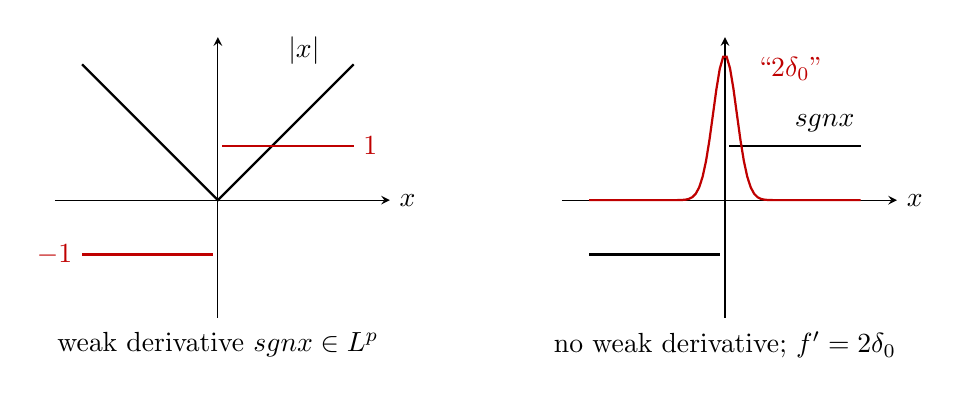
\begin{tikzpicture}[scale=1.15, >=stealth]
    \begin{scope}
        \draw[->] (-1.8,0) -- (1.9,0) node[right] {$x$};
        \draw[->] (0,-1.3) -- (0,1.8);
        \draw[thick] (-1.5,1.5) -- (0,0) -- (1.5,1.5);
        \node at (0.95,1.65) {$|x|$};
        \draw[thick, red!75!black] (0.05,0.6) -- (1.5,0.6);
        \draw[thick, red!75!black] (-1.5,-0.6) -- (-0.05,-0.6);
        \node[red!75!black, right] at (1.5,0.6) {$1$};
        \node[red!75!black, left] at (-1.5,-0.6) {$-1$};
        \node[below] at (0,-1.35) {weak derivative $\operatorname{sgn} x \in L^p$};
    \end{scope}
    \begin{scope}[xshift=5.6cm]
        \draw[->] (-1.8,0) -- (1.9,0) node[right] {$x$};
        \draw[->] (0,-1.3) -- (0,1.8);
        \draw[thick] (0.05,0.6) -- (1.5,0.6);
        \draw[thick] (-1.5,-0.6) -- (-0.05,-0.6);
        \node at (1.1,0.85) {$\operatorname{sgn} x$};
        \draw[thick, red!75!black, domain=-1.5:1.5, samples=80] plot (\x, {1.6*exp(-30*\x*\x)});
        \node[red!75!black, right] at (0.25,1.45) {``$2\delta_0$''};
        \node[below] at (0,-1.35) {no weak derivative; $f' = 2\delta_0$};
    \end{scope}
\end{tikzpicture}
